% vim:ft=tex:
%
\documentclass[12pt]{article}

\usepackage{outlines}
\usepackage{graphicx}

\title{TedChat - Phase 1}
\author{Andrew Kao\\ Cory Knapp}

\begin{document}
\maketitle

\section{Introduction}
	This document describes the design and security properties of TedChat, a
	secure desktop chat application.  TedChat is written by TeamTed, which is
	composed of Andrew Kao and Cory Knapp, as an exercise in implementing
	secure protocols. As a result, the product emphasises security over all
	else.
		
\section{Application Properties}
	TedChat is designed to securely send messages composed of text between two client applications.

\section{Client Design Overview}
The client application is to be designed in c++ using the Qt framework

In figure \ref{fig:client_window} we see a mock up of the main client window
and a corresponding table describing it's features in table
\ref{tab:client_window_feat}.  Likewise, a mock up of the dropdown menu can be
seen in \ref{fig:client_dropdown} 
and a corresponding table describing it's features in table
\ref{tab:client_dropdown_feat}.  

Not pictured in a figure is the preferences interface, which as of now, consists 
as a single field for entering the user's ID.

\begin{figure}[htpb]    
\label{fig:client_window}	
\caption{Client Window}
\centering
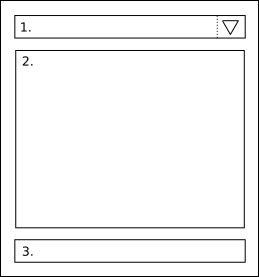
\includegraphics[width=0.5\textwidth]{client_window}
\end{figure}


\begin{table}[htpb]
	\centering
	\caption{Description of Client Window Features}
	\label{tab:client_window_feat}
	\begin{tabular}{|l|p{8cm}|}
	\hline
		1 & Text field and drop down menu to display and change the active chat
		channel\\
	\hline
		2 & Text field to show recent chat history\\
	\hline
		3 & Text field to compose new messages\\
	\hline
	\end{tabular}
\end{table}

\begin{figure}[htpb]    
\label{fig:client_dropdown}
\caption{Conversation Selection Dropdown}
\centering
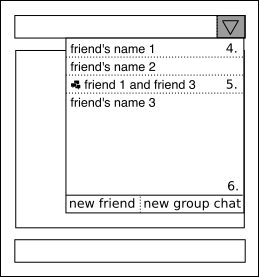
\includegraphics[width=0.5\textwidth]{client_dropdown}
\end{figure}

\begin{table}[htpb]
	\centering
	\caption{Description of Client Window Drop Menu}
	\label{tab:client_dropdown_feat}
	\begin{tabular}{|l|p{8cm}|}
	\hline
		4 & Recent friends are stored in a list in the top of the menu\\
	\hline
		5 & Group chats are shown as a list of names and denoted with an icon\\
	\hline
		6 & the options for adding new friends, or iniilzing a new group chat
		appear at the bottom of the menu\\
	\hline
	\end{tabular}
\end{table}

\section{RESTful Server Design Overview}
The server will be based on a SQL database.  We can neglect to include a table
to track user information; from the server's perspective, each user is
represented by a single identification number.  However, it is desirable
(though not strictly necessary) to insure that users are assigned unique
identification numbers.  This will be implemented using a table consisting of a
one column and a one row.  We'll track the ID of the user most recently
registered, and increment it when a new user ID is requested.

The message table will consist of four fields:
\begin{outline}[enumerate]
	\1 \textbf{Sender ID} - The self reported ID number of the user claiming to
		be the message sender.

	\1 \textbf{Recipient ID} - The ID number of the message's intended recipient.

	\1 \textbf{Timestamp} - Date and time that the message was posted to the
		server.  This field is not provided by the client; the timestamp is
		generated by the server.

	\1 \textbf{Ciphertext} - Encrypted message, including message meta data.
\end{outline}

\section{Assets/Stakeholders}

Because of the relatively limited scope of the product, there are few assets to
protect.  The primary assets are the messages sent between users.  The primary
goal is to protect the messages confidentiality and integrity. Secondly, we
must maintain control of the server to ensure the availability of messages to
the user.  Thus, control of the server is also an Asset that requires
protection.

The primary stakeholder in this scenario is the user who expects
their messages to be sent securely, and without interruption.

\section{Adversarial Model}

The primary concern is to guard against a man in the middle attack.  It is
imperative that an attacker who is able to intercept any message find that
message useless.  By useless, we mean that the attacker should be unable to
discern any meaning from the cipher text, nor should they be able to construct
meaningful alternate cipher text as a substitute. 

Notice that the server does no authentication of users at any time.  User 1
may, with ill intentions, request a messages from the server which are intended
for user 2.  However, without user 2's private key, this message will be
unreadable.

A second troubling scenario would be the case where a user sends a message
posing as another user.  Imagine that user 1, 2 and 3 are all friends, and of
course each user has the other two's public keys.  It would be easy for user 1
to post a message to the server with user 2 as the reported sender and user 3
as the recipient.  However, user 2 and 3 generated a shared secret key through
a Diffie-Hellman key transfer when they first connected.  Any genuine message
from user two will contain in it's metadata the shared secret, and others can
be rejected as inauthentic. 

\section{Previous work }
\begin{enumerate}

\item WhatsApp Whitepaper
\item OpenSSL Documentation
\item PGP Documentation
\item TLS
\item Let’sEncrypt
\item QT Documentation

\end{enumerate}

\subsection{Security Model}
\label{sub:security_model}
\begin{figure}[h]
\caption{Handshake}
\label{fig:handshake}
\centering
\includegraphics[width=0.9\textwidth]{handshake}
\end{figure}

\begin{figure}[h]
\caption{Message Decryption}
\label{fig:message_decryption}
\centering
\includegraphics[width=0.9\textwidth]{message_decryption}
\end{figure}

\begin{figure}[h]
\caption{Message Encryption}
\label{fig:message_encryption}
\centering
\includegraphics[width=0.9\textwidth]{message_encryption}
\end{figure}

\begin{figure}[h]
\caption{Session Keys}
\label{fig:session_keys}
\centering
\includegraphics[width=0.9\textwidth]{session_keys}
\end{figure}

\begin{figure}[h]
\caption{Shared Secret}
\label{fig:shared_secret}
\centering
\includegraphics[width=0.9\textwidth]{shared_secret}
\end{figure}

\begin{figure}[h]
\caption{Updating Session Keys}
\label{fig:updating_session_keys}
\centering
\includegraphics[width=0.9\textwidth]{updating_session_keys}
\end{figure}
\begin{outline}[enumerate]
\1 Initialization

	\2 When user installs application, the program will generate their
	Curve25519 public-private key pair.

\1 Connection to server

	\2 User registration

		\3 Server will generate a UUID and assign it to user

\1 User-user handshake

		\2 Passing Public Key (see figure \ref{fig:handshake})

		\3 Users will physically pass their public key and user ID to users
		they wish to chat with.

\1 Creating the chat

		\2 Shared secret (see figure \ref{fig:shared_secret})

		\3 Both users will calculate a shared secret using Elliptic Curve
		Diffie-Hellman (ECDH) on their public-private key pairs.

	\2 Generate session keys (see figure \ref{fig:session_keys})


		\3 Both users generate their respective initial root keys from the
		shared secret using HKDF.

		\3 Both users generate their respective initial chain keys from their
		respective root keys using HKDF.

		\3 Both users generate their respective initial message keys from their
		respective chain keys using HMAC-SHA256.

\1 Encryption/Decryption

	\2 Encryption (see figure \ref{fig:message_encryption})


		\3 When a user sends a message, a message key will be generated from
		the chain key The user generates an ephemeral Curve25519 public key.

		\3 The chain key will ratchet up by one.

		\3 The user encrypts the message key with the public key of the
		recipient with RSA.

		\3 The user appends the encrypted message key to the encrypted message
		with PGP.

		\3 The user concatenates the encrypted message, encrypted key, and
		ephemeral key together and sends the whole string to the recipient.

	\2 Decryption (see figure \ref{fig:message_decryption})

		\3 The user uses their private key to decrypt the message key.

		\3 The user uses the message key to decrypt the message.

\1 Updating Session Keys (see figure \ref{fig:updating_session_keys})

	\2 A user will use the same root key until a response is received.

	\2 When a response is received, the user will generate a new ephemeral
	public key and generate an ephemeral secret by using ECDH on his new
	ephemeral public key and the other user’s ephemeral public key that was
	advertised in the response.

	\2 The user will then generate new root and chain keys from the
	ephemeral secret.
\end{outline}




\section{Analysis}

\subsection{Message Security}
Because each message is encrypted by a key that is also encrypted with the
recipient’s public key, an adversary cannot know the message key (and thus
cannot decrypt the message) without knowing the recipient’s private key.

\subsection{Forward Secrecy}
Our system ensures that no message keys are recycled, therefore an adversary
would not be able to use a compromised message key to decrypt past messages.

\subsection{Server}

OpenSSL/TLS comes with client certificate authentication for our server, so
User 1 would not be able to make requests to the server for User 2's messages.
This also means User 1 would not be able to send a message to User 3 posing as
User 2. In the event that an adversary were to successfully pose as User 2 or
for some reason SSL/TLS authentication is compromised, the impostor will not be
able to decrypt User 2's messages without User 2's private key, and he does not
know the shared secret of the actual User 2 and User 3, so User 3 would not
accept any messages from the impostor.

\end{document}
